\documentclass[11pt,twoside,a4paper, titlepage]{article}
\usepackage{xcolor}
\usepackage{soul} %\hl
\usepackage[T1]{fontenc}
\usepackage{graphicx}

\begin{document}
\title{Counter Hack Notes}
\author{Gautam Batra}
\date{\today}
\maketitle

\section{Important Commands}
\begin{center}

  \begin{tabular}[c]{|p{3cm}|p{8cm}|} \hline
    \textbf{Command} & \textbf{Use} \\
    \hline
    netstat -na & show port status, n=numerical form, a=all \\
    \hline
    chkconfig & list the names of services started by init, and those started by inetd/xinetd \\
    \hline
    lsof & list open files: lists the files opened for each process lsof\textbar grep [prog\_name]: to see files specific to a program lsof -p [pid]: lists files opened by the process denoted by the PID lsof -i: lists the tcp and udp usage \\
    \hline
    /etc/passwd & Contains information about each user (one user per line). If (encrypted) passwords not mentioned, * or x will be displayed. Passwords will be stored in the shadow password file: /etc/shadow or /etc/secure \\
    \hline
    s/etc/group & contains information about the groups \\
    \hline
    find / -uid 0 -perm -4000 -print & find all SetUID programs \\
    \hline
    rsh, rlogin, rcp & remote shell/login/copy. unsecured (clear text). dont use. \\
    \hline
  \end{tabular}
\end{center}

\section{Notes}
\begin{itemize}
  \item  TCP Control bits: \textbf{U}nskilled \textbf{A}ttackers \textbf{P}ester \textbf{R}eal \textbf{S}ecurity \textbf{F}olks
  \item  Find all SYN packets tcpdump `tcp[13] \& 2 != 0'
  \item  IP Tables: Blocking an IP: \\
    \hspace*{1cm}iptables -A INPUT -s 192.168.1.5 -j DROP 
  \item  A port with a listening service is known as an open port, whereas a port where nothing is listening is closed.
  \item  inetd: internet daemon
  \item  /etc/services: contains list of all network services and port numbers
  \item /etc/inetd.conf: for configuring individual network services\\
    \hspace*{1cm}wait status: wait = one process for all requests of a service \\
    \hspace*{3cm} nowait = inetd creates one process per request
    \begin{figure}[!hbp]
      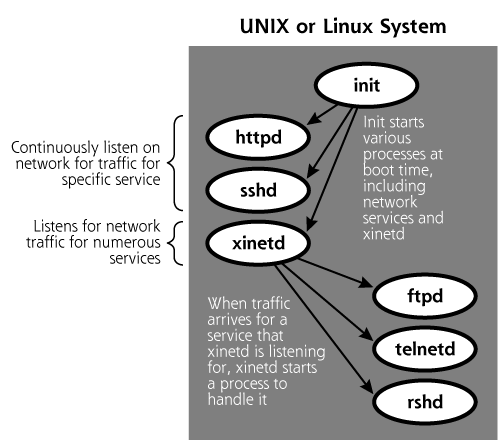
\includegraphics[scale=0.5]{images/services.png}
      \caption{Relationship between init, xinetd, and various network services \label{fig_services}}
    \end{figure}
  \item chkconfig -{}-list: display a list of all services configured to start up at system boot and by xinetd
\end{itemize}
\end{document}
